\documentclass[a4paper]{report}
\usepackage[english]{babel}
\usepackage[utf8]{inputenc}
\usepackage[T1]{fontenc}
\usepackage{subfig}
\usepackage{caption}
\usepackage{subcaption}
\usepackage{anysize}
\usepackage[a4paper,top=3cm,bottom=2cm,left=2cm,right=2cm,marginparwidth=1.75cm]{geometry}

\usepackage{amsmath}
\usepackage{amssymb}
\usepackage{dsfont}
\usepackage{derivative}
\usepackage{graphicx,fancyhdr,titlesec,color, wrapfig}
\usepackage[colorlinks=true, allcolors=blue]{hyperref}
\usepackage{sectsty}
\usepackage{apacite}
\usepackage{float}
\usepackage{titling} 
\usepackage{blindtext}
\usepackage[numbers]{natbib}
%\setcitestyle{numbers,open={[},close={]}}
\bibliographystyle{unsrtnat}
%\usepackage[colorinlistoftodos]{todonotes}
\graphicspath{{images/}}
%%%%%%%%%%%%%%%%%%%%%%%%%%%%%%%%%%%%%%%%%%%%%%%%%%%%%%%%%%%%%%%%%%%%%%%%%%%%%%%%%%%%%%%%%%%%%%%%%%%
\definecolor{gray75}{gray}{0.75}
\newcommand{\hsp}{\hspace{20pt}}
\titleformat{\chapter}[hang]{\Huge\bfseries}{\thechapter\hsp\textcolor{gray75}{$\mid$}\hsp}{0pt}{\Huge\bfseries}
\pagestyle{fancy}
\fancyhead{}
\fancyhead[RO,LE]{Implementation of a QAOA for the Max-Cut problem}
\fancyfoot{}
\fancyfoot[LE,RO]{\thepage}
\fancyfoot[LO,RE]{Part \thechapter}
\usepackage{listings}
%%%%%%%%%%%%%%%%%%%%%%%%%%%%%%%%%%%%%%%%%%%%%%%%%%%%%%%%%%%%%%%%%%%%%%%%%%%%%%%%%%%%%%%%%%%%%%%%%%%%
\usepackage{tikz}
\usetikzlibrary{quantikz, shapes.geometric, arrows, petri, topaths}

%\usepackage[position=top]{subfig}
%\renewcommand{\thesubsection}{\thesection.\alph{subsection}}
\usepackage{biblatex}
\addbibresource{others/references.bib}

\setlength{\parskip}{1em}

\begin{document}
    \begin{titlepage}

\newcommand{\HRule}{\rule{\linewidth}{0.5mm}} 							% horizontal line and its thickness
\center 
 
\includegraphics[width=0.6\textwidth]{images/TU_delft_logo.jpg}\\[1cm]   % University logo
% University
\textsc{\LARGE Delft University of Technology}\\[1cm]

% Document info
\textsc{\Large Quantum Information Project}\\[0.2cm]
\textsc{\large AP3421-PR}\\[1cm] 										% Course Code
\HRule \\[0.8cm]
{ \huge \bfseries Quantum Approximate Optimization Algorithm for the Max-Cut problem}\\[0.7cm]								% Assignment
\HRule \\[2cm]
\large
\emph{Authors:}\\Smit Chaudhary (5273900)\\Ignacio Fernández Graña (5358809)\\Mastrodomenico Luigi Pio (5316197)\\[1.5cm]												
{\large \today}\\[5cm]

\vfill 

\end{titlepage}
    \tableofcontents
\chapter{The Max Cut problem}
    In this section, we introduce the problem that we solve.
We first define the problem with particular focus on defining the cost function in a manner that would translate well to the quantum strategy we later employ.
%%%%%%%%%%%%%%%%%%%%%%%%%%%%%%%%%%%
\section{The Max Cut problem}
Consider an unweighted un-directional graph $G := (V, E)$. $V$ is the set of vertices (or nodes) of the graph while $E$ is the set of edges.
Consider a partition of the vertices into two disjoint subsets, namely, set $A$ and set $B$.
Any general partition of the vertices will potentially have edges such that the two nodes at the end of the edge are in different subsets.
Thus, the partition boundary can be said to have \textit{cut} the edge.
Let the number of edges being cut by a partition $i$ be $C_i$.
The \textbf{MaxCut} problem is to find the partition for any given graph $G$ such that the $C_i$ is maximum.
Thus, we want to find the partition that crosses the maximum number of edges.

It is instructive to look at the nature of the problem and the solution space here.
The problem is to optimize a certain function (number of edges being crosses by the partition) under certain conditions (the graph G).
One partition varies from other partition in terms of the combination of nodes chosen to be together in one subset.
Thus, the solution space is all possible partitions, which are all possible combinations of the nodes.
This means, the solution space is discrete.
Problems of this kind are called \textit{combinatorial optimization problem}.

The discrete solution space grows extremely rapidly with the size of the graph that we consider.
The solution space grows as $\mathcal{O}(2^n)$ where $n$ is the number of nodes in the graph.
Thus, for large graphs, the simplest solution, that is, checking all partitions is very costly.
There are other better classical algorithms but the problem remains very difficult and costly to solve.
In fact, MaxCut is an NP-Hard problem. Thus finding a solution for a general graph G is not possible.
Approximate algorithms that run in polynomial time do however exist.

%%%%%%%%%%%%%%%%%%%%%%%%%%%%%%%%%%%
\section{Mathematical Formulation}

Let us define a function that identifies which subset any particular node is in. We define a function
\begin{equation}
     g(i) = \begin{cases} 
         1 & i \in A \\
        -1 & i \in B 
   \end{cases}
   \label{g_def}
\end{equation}
Thus, for any edge with vertices $i$ and $j$, if it is being cut by the partition or not can be given by
\begin{equation}
    C_{ij} = \frac{1}{2}(1 - g(i)g(j))
    \label{C_def}
\end{equation}
Consequentially, the total number of edges being cut is simply the sum of $C_{ij}$ over all edges. Thus, the function that we want to maximize is

$$C(g) = \sum_{(i, j) \in E}C_{ij} = \frac{1}{2}\sum_{(i, j) \in E}(1 - g(i)g(j))$$

Here, $g$ can be seen as a string of length n where the $g_i = g(i)$.
We will use this idea when we implement the quantum algorithm.

\begin{figure}[h]
    \centering
    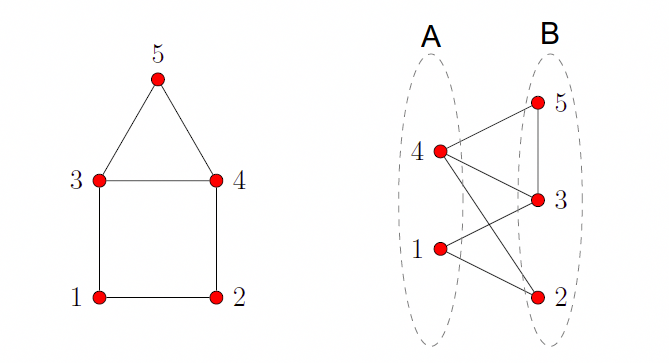
\includegraphics[scale=0.65]{images/GraphCut.png}
    \caption{A 5 node graph with one possible partition of the nodes.}
    \label{fig:GraphCut}
\end{figure}

As an illustration, let us consider a 5 node graph with the connectivity as shown in the figure \ref{fig:GraphCut} above.
Additionally, say we have the partition in two sets, namely $A$ and $B$ as shown in the figure.
For this particular partition, the number of edges being cut are 5.
Note that, for any partition, there exists another partition with all the nodes between the two exchanged.
These two partitions would have the same number of edges being cut.

Having established the problem, next we look at the algorithm to solve it.
\chapter{QAOA}
    The Quantum Approximate Optimization Algorithm (QAOA) is a class of hybrid quantum-classical approximate algorithms which can tackle combinatorial optimization problems \cite{farhi2014quantum, alam2019analysis}.
QAOA combines the preparation of a quantum state and the properties of superposition with classical optimization.
As is in the name, it is also an approximate algorithm thus it does not necessarily give the optimal solution (the actual partition with MaxCut in our case) but gives an approximation of such a solution.

At the current stage of development of Quantum Computing infrastructure, called \textit{Noisy Intermediate Scale Quantum} era or NISQ era, QAOA are of particular interest.
There has been considerable interest already in developing use cases within the limits of currently available quantum computers as well as projecting the kind of quantum advantage we might be able to achieve in near term \cite{Guerreschi_2019}.
As has been shown in contemporary works \cite{8957201} as well, we also look at the limitations of QAOA using the currently available quantum computers.

Nevertheless, QAOA remains a very prominent line of thought regarding new quantum algorithms and has a wide applicability across different fields.
It can be used to solve problems in academia \cite{Bengtsson_2020}, in logistics \cite{Vikst_l_2020}, finance etc.

In this project, we look at one combinatorial optimization problem, namely the MaxCut problem as stated earlier.
We analyse the working of the algorithm in an ideal case.
We also employ simple noise models and see how the presence of noise affects the performance of the algorithm.
Further, we implement the algorithm on actual hardware backend and analyse the performance and discuss the limitations of the noisy systems we currently have.

%%%%%%%%%%%%%%%%%%%%%%%%%%%%%%%%%%%%
\section{The algorithm}

As described above, the function that we want to maximize is $C(z)=\sum_{k=1}^m C_k(z)$, with $m=|E|$ being the number of edges in the graph.
Here, $z=z_1z_2\cdots z_n$ and $z_i\in \{0,1\}$ based on which node is in which subset.
Thus, here, we encode the information about the subset a particular node belongs to by $0$ and $1$ unlike $1$ and $-1$ as discussed in last section.
$C_k \in \{0, 1\}$ based on the string $z$. It tells us if the $k^{th}$ edge is being cut or not by the partition denoted by the string $z$.
Our aim is to find the string(s) $z$ that give us the maximum value of $C$.

Firstly, we need to convert this (thus far) classical problem into a quantum problem. Thus, the string $z$ which denotes a particular partition of the nodes, translates to the quantum state $\ket{z}$.

To illustrate this, the partition shown in the figure \ref{fig:GraphCut}, would be denoted by the classical string $z = 01101$ and subsequently, in the quantum state $\ket{01101}$.
Thus, each of the basis state would denote a particular partition of the nodes.

Further, the cost function that we defined above and which we want to maximize, can then be represented as an operator.
We define it such that acting on any basis state (each of which now denotes a partition), it gives back the same basis state but multiplied with the the cost $C(z)$ of that basis state.
Thus, the basis states are the eigenstates with he cost as their corresponding eigenvalues. This can be expressed as
\begin{equation}
    \hat{C}\ket{z}= \sum_{k=1}^m \hat{C}_k\ket{z} = c(z)\ket{z}
    \label{equation:cost_op}
\end{equation}

For the operator $C$, there will be a specific value $c'=c(z')\geq c(z),\forall z\neq z'$ which will be the solution of our maximization problem.
For any general state $\ket{\psi}=\sum_{z \in\{0,1\}^n}a_z\ket{z}$, we can construct the expectation value of the cost function as:

\[
    \left\langle C\right\rangle =\bra{\psi}\hat{C}\ket{\psi} = \sum_{z \in\{0,1\}^n}c(z)|a_z|^2
\]

Thus, to find an approximate solution, we try to find $\ket{\psi}$ that maximizes $\langle C \rangle$

Say the actual MaxCut partition is $z^*$, then, we want to get $\ket{\psi} = \ket{z^*}$.
In that case, $\langle C \rangle = \langle C \rangle_{max}$.
But in general, we don't know how to find $\langle C \rangle_{max}$ efficiently.
Thus, what we do is we try and get $\langle C \rangle$ as close to $\langle C \rangle_{max}$ as possible.
In other words, we try to get $\ket{\psi}$ such that the amplitude(s) of $\ket{z^*}$ is very high.

As a metric of performance, we define the approximation ratio denoted by $r$ and defined as
$$r = \frac{ \langle C \rangle }{\langle C \rangle_{max}} $$


Having established our goal to get a $\ket{\psi}$ with high amplitudes for $\ket{z^*}$, let us define the quantum operators that we use.
%%%%%%%%%%%%%%%%%%%%%%%%%%%%%%%%%%%
\subsection{First step: $U_C(\gamma)$}
Firstly, we define a Hamiltonian called the \textit{Cost Hamiltonian} and we denote it by $H_C$.
This is essentially the function $C$ that we defined earlier.
Thus, it can be written as

\[
    H_C = \sum_{k=1}^m C_k = \sum_{x \in \{0, 1\}^n}C(x)\ket{x}\bra{x}
\]
As we can see it is the same operator that we defined in \ref{equation:cost_op} and it has the same properties.
Using this Hamiltonian, we define a Unitary operator $U_C(\gamma)$ in the following way:
$$U_C(\gamma) = e^{-i \gamma H_C}$$

Thus, $U_C$ is a parametric operator, parameterised by the real number $\gamma$

Now let's see what is the action of this operator on a general state $\ket{\psi}$
\[
    U_C(\gamma)\ket{\psi}= U_C(\gamma)\sum_{z \in\{0,1\}^n} a_z\ket{z} = \sum_{z \in\{0,1\}^n} a_z e^{-i\gamma C(z)} \ket{z}
\]

Thus, all basis states get a phase depending on the cost of the partition corresponding to that state and $\gamma$.
%%%%%%%%%%%%%%%%%%%%%%%%%%%%%%%%%%%%
\subsection{Second step: $U_B(\beta)$}
The amplitudes change, however, since the only change is in the complex phases of the states, the probabilities for each state are however same as before applying the operator $U_C$ and likewise, the expectation values have not changed either.

Having changed the relative phases of the states, we need to operate with an operator that now mixes them, that is, causes a superposition between these states.
To achieve this, as earlier, we first define an Hamiltonian and call it the \textit{Mixing Hamiltonian}.
We define it as following:

\[
    H_B=\sum_{k=1}^n\sigma_k^x= \sigma_1^x\otimes \mathbb{I}^{\otimes(n-1)} + \mathbb{I} \otimes \sigma_2^x \otimes \mathbb{I}^{ \otimes(n-2)}+ \cdots + \mathbb{I}^{\otimes(n-1)} \otimes \sigma_n^x
\]

Again using this Hamiltonian, we define a unitary $U_B(\beta)$ as
$$U_B(\beta)= e^{-i\beta H_B}$$

As earlier, $U_B(\beta)$ too is a parametric operator that is parameterised by real number $\beta$.

To see the action of this operator, we write $U_B(\beta)$ as

\[
    U_B(\beta)= e^{-i\beta H_B} = e^{-i\beta\sum_{k=1}^n \sigma_k^x} = \prod_{k=1}^n e^{-i\beta \sigma_k^x}
\]

Recalling the definition of the $x$-rotation operator $R_x(\theta)=e^{-i\frac{\theta}{2}\sigma^x}$, with 

$\theta\in [0,2\pi]$, it becomes clear that the operator $U_B(\beta)$ can be written as:
\[
    U_B(\beta)= R_x^{\otimes n}(2\beta)\quad\text{with }\beta\in [0,\pi]
\]

Thus, this is actually rotation about X for each qubit by an angle $2\beta$.

The combined effect of applying $U_C(\gamma)$ followed by $U_B(\beta)$ is to first give a complex phase to all the states (which depends on the cost and the parameter $\gamma$) followed by applying an X rotation (which depends on the parameter $\beta$) for all qubits.

So, all the states will mix and how exactly they mix is controlled by $\gamma$ and $\beta$.
We try and tweak these parameters such that this mixing happens in such a way that the amplitude of the states with low cost falls (they interfere destructively) and the amplitudes of the states with higher cost rises (they interfere constructively).

\subsection{Building the operators}
Having defined the operators mathematically, it is instructive to look at how we implement the operators.

From the definition and action of $U_B(\beta)$ as indicated in the previous subsection, it is rotation about X axis by an angle $2\beta$ for each qubit. Thus, it can be implemented using $n$ single qubit rotations where $n$ is the number of qubits (thus, also the number of nodes). Thus,

$$U_B(\beta)=\prod_{i=1}^{n} R_{Xi}(2\beta)$$

Now, looking at $U_C(\gamma)$, and the definition of $H_C$ and the equations \ref{g_def} and \ref{C_def} along with the fact that $\ket{z}$ denotes the partitions, we define:

$$H_C = \sum_{(jk) \in E} \frac{1}{2}(\mathbb{I}- Z_j Z_k)$$

The implementation of $U_C(\gamma)$ would then translate to 

$$U_C (\gamma) = \prod_{(i,j) \in E} CR_Z_{i,j}(-2\gamma)R_{Zi}(\gamma)R_{Zj}(\gamma)$$
$i$ and $j$ are the nodes at the end of the edge. $CR_Z_{i,j}(-2\gamma)$ is a controlled rotation around Z by angle $2\gamma$, and $R_Z_{i}(\gamma)$ is rotation about Z by angle $\gamma$ for qubit $i$. We would have to apply this combination for each edge in $E$.

To see the implementation for a simple graph, consider a regular 3-node graph. The graph is as shown in figure \ref{fig:triangle}.

\begin{figure}[h]
    \centering
    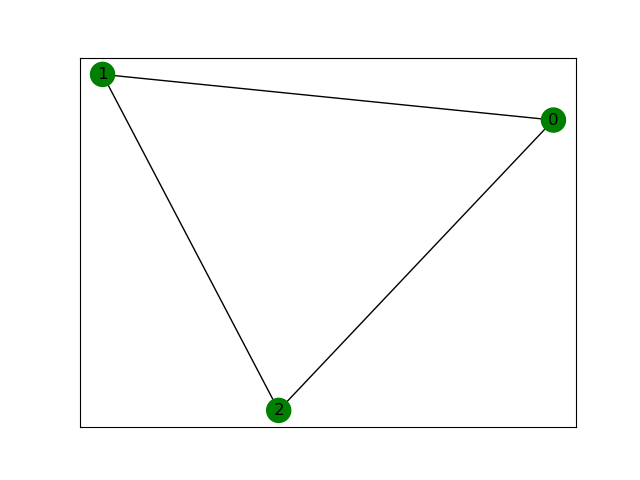
\includegraphics[scale=0.5]{images/triangle.png}
    \caption{A regular 3-node graph.}
    \label{fig:triangle}
\end{figure}

To implement QAOA for this graph, we would have to apply the following gates as shown in figure \ref{fig:3ncircuit}

\begin{figure}[h]
\begin{center}
    \begin{quantikz}
        \lstick{$\ket{+}$}  & \ctrl{1}\gategroup[wires=3,steps=6,style={inner sep=6pt}]{$U_C$} & \gate{R_Z(\gamma)} & \qw & \qw & \ctrl{2} &  \gate{R_Z(\gamma)} &\qw & \gate{R_X(2\beta)}\gategroup[wires=3,steps=1,style={inner sep=6pt}]{$U_B$} &\meter{} &\cw \\
        \lstick{$\ket{+}$}  & \control{} & \gate{R_Z(\gamma)} & \control{} & \gate{R_Z(\gamma)} & \qw & \qw &\qw &\gate{R_X(2\beta)} & \meter{} & \cw\\
        \lstick{$\ket{+}$}  & \qw & \qw  & \ctrl{-1} & \gate{R_Z(\gamma)} & \control{} & \gate{R_Z(\gamma)} &\qw &\gate{R_X(2\beta)} & \meter{} & \cw
    \end{quantikz}
%    \includegraphics[width=1\linewidth]{circuit.png}
    \caption{Circuit for the 3-n regular graph with the final measurement in the computational basis}
    \label{fig:3ncircuit}
\end{center}
\end{figure}


Note that the circuit on figure \ref{fig:3ncircuit} is not optimal. Since all gates commute, the circuit could be compiled with many less gates. Nevertheless, for the sake of simplicity, we will stick to this ansatz as this allows to easily generalize for different graphs.

It would be insightful to talk about the particular structure of $U_B$ or rather its relation to $U_C$.
Note that here, the gates in $U_C$ and those in $U_B$ do not commute.
By extension, $U_C$ and $U_B$ themselves do not commute.
This is an important feature.

To illustrate this, let us see what would happen in case we defined $H_B$ and by extension $U_B$ in the same manner but instead of having the rotation about X axis, we rotated about Z axis.
First, it is clear that in that case, $U_C$ and $U_B$ would commute. But why is this undesirable?

From our discussion earlier, we know that $U_C$ applies phase to all states, thus it does not change the probabilities.
If $U_B$ were to commute with it, then that means, $U_C$ and $U_B$ would have the same eigenbasis.
And in that case, applying $U_B$ to the eigenstates of $U_C$ (which are the standard basis states), one would get

$$U_B(\beta)\ket{z} = b(z)\ket{z}$$

since these are also the eigenstates of $U_B$. And since, $U_B$ is a unitary matrix, the eigenvalues are all of unit magnitude. Thus, applying $U_B$ is same as applying some phase.

All of this would mean that the amplitudes of the states change but they change only in terms of the phase they have.
And thus, the probabilities of these states are unchanged.

This means, $\langle C \rangle$ which we want to maximise, never changes, no matter what values of $\gamma$ and $\beta$ we choose.
Thus, it is crucial that $U_B$ and $U_C$ do not commute since the only purpose of $U_B$ is to mix the states (thus the name \textit{Mixing Hamiltonian} for $H_B$) and that would not be possible if they commute.
This means, we could choose rotations about $Y$ instead of $X$ for $H_B$ but not about $Z$ or anything that commutes with $U_C$ 

\section{Workflow}

Having defined the necessary operators, we have a look at the algorithm now.
We start with a state that is equal superposition of all states. Thus we start with:

\[\ket{\psi}=H^{\otimes n}\ket{0}^{\otimes n} = \frac{1}{\sqrt{2^n}}\sum_{z \in\{0,1\}^n}\ket{z}\]

On this initial state, we apply $U_C(\gamma)$ followed by $U_B(\beta)$.
Let us say, we do this for $p$ times.
Thus we have $2p$ parameters, i.e, $p$ values of $\gamma$ and $p$ values of $\beta$.
From here on, we call one application of $U_C$ followed by $U_B$ a layer.
Thus, we here have $p$ layers.

After applying the unitary transformations, we measure the qubits in standard basis to get the state $z$ and from that, we get the cost for that state i.e, $C(z)$.

Thus, the circuit can be represented as in the figure \ref{fig:General_QC} below

\begin{figure}[h]
    \centering
    \begin{quantikz}
        \lstick[wires=4]{$\ket{0}^{\otimes n}$} & \gate{H} & \gate[wires=4]{U_C(\gamma_1)}\gategroup[4,steps=2,style={dashed,
        rounded corners,fill=blue!20, inner xsep=2pt},
        background,label style={label position=below,anchor=
        north,yshift=-0.2cm}]{{$1^{st}$ layer}} & \gate[wires=4]{U_B(\beta_1)}& \ \ldots\ \qw & \gate[wires=4]{U_C(\gamma_p)}\gategroup[4,steps=2,style={dashed,
        rounded corners,fill=blue!20, inner xsep=2pt},
        background,label style={label position=below,anchor=
        north,yshift=-0.2cm}]{{$p^{th}$ layer}} & \gate[wires=4]{U_B(\beta_p)}& \meter{} & \cw\rstick[wires=4]{Measure\\results}\\
        & \gate{H} & & & \ \ldots\ \qw & & &\meter{} & \cw \\
        &\wave & & & & & & & &\\
        & \gate{H} & & & \ \ldots\ \qw & & &\meter{} & \cw 
    \end{quantikz}
    \caption{This is a general representation of the quantum circuit for $n$ qubits and $p$ layers.}
    \label{fig:General_QC}
\end{figure}



We start with arbitrary values of the $2p$ parameters for the operators.
The state just before measurement is denoted as $\ket{\gamma, \beta}$, which would be:
\[
    \ket{\gamma,\beta} = U_B(\beta_p)U_C(\gamma_p)\cdot\cdot\cdot U_B(\beta_2)U_C(\gamma_2)\cdot U_B(\beta_1)U_C(\gamma_1)\cdot H^{\otimes n}\ket{0}^{\otimes n}
\]
\[\text{with }\gamma = [\gamma_1,\gamma_2,...\gamma_p] \text{ and }\beta = [\beta_1, \beta_2,...\beta_p] \text{,}\]

Upon measurement, we get state $\ket{z}$ for which we can calculate its \emph{cost} $C(z)= \sum_{k=1}^m C_k(z)$.
We do multiple runs of the algorithm to get the expectation value $ \langle C \rangle$.
We want $ \langle C \rangle = \bra{\psi(\beta, \gamma)}C(z)\ket{\psi(\beta, \gamma)}$ to be maximum.
Thus, we feed this to a classical optimizer, which returns updated values of the circuit parameters \textbf{$(\beta, \gamma)$}.
This is not part of the \textit{quantum} algorithm but merely classical optimization of the control parameters.
The choice of optimizer is discussed later.
The measurement which gives the highest cost can then be taken as the solution.
It is shown by Farhi et. al \cite{farhi2014quantum} that for $p \rightarrow \infty$, we would surely find the global maximum of $ \langle C \rangle$.

The algorithm can be summarised using the schematic in figure \ref{fig:Flow_QAOA}

\begin{figure}[h]
    \centering
    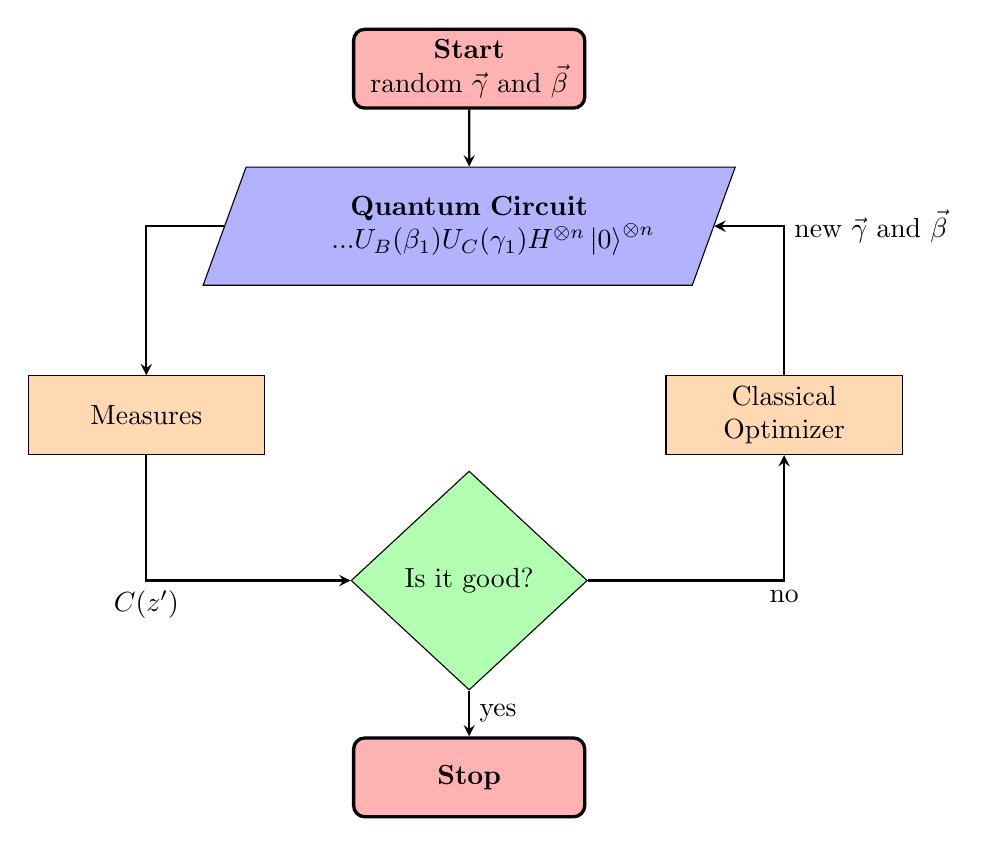
\begin{tikzpicture}[node distance=2cm]
    
        \tikzstyle{startstop} = [rectangle, rounded corners, minimum width=2cm, minimum height=1cm,text centered, text width=2.7cm, draw=black, fill=red!30, very thick]
        \tikzstyle{Q-startstop} = [rectangle, rounded corners, minimum width=5cm, minimum height=2cm,text centered, text width=4.5cm, draw=black, fill=blue!30]

        \tikzstyle{Q-io} = [trapezium, trapezium left angle=70, trapezium right angle=110, minimum width=1.7cm, minimum height=1.5cm, text centered, text width=3.5cm, draw=black, fill=blue!30]
        \tikzstyle{process} = [rectangle, minimum width=3cm, minimum height=1cm, text centered, text width=2.5cm, draw=black, fill=orange!30]
        \tikzstyle{decision} = [diamond, minimum width=3cm, minimum height=1cm, text centered, text width=2cm, draw=black, fill=green!30]
        \tikzstyle{arrow} = [thick,->,>=stealth]
        
        \node (start)[startstop] {\textbf{Start}\\ random $\vec{\gamma}$ and $\vec{\beta}$};
        \node (QC) [Q-io, below of=start, yshift=0cm] {\textbf{Quantum Circuit}\\     $...U_B(\beta_1)U_C(\gamma_1) H^{\otimes n}\ket{0}^{\otimes n}$};
        \node (dec1) [decision, below of=QC, yshift=-2.5cm] {Is it good?};
        %\node (density) [process, left of=dec1, xshift=-2.1cm] {Probability\\Density};
        \node (measures) [process, left of=dec1, xshift=-2.1cm, yshift=2.1cm] {Measures};
        %\node (optimization) [process, right of=dec1, xshift=2cm]{Classical Optimization};
        \node (update)[process, right of=dec1, xshift=2cm, yshift=2.1cm]{Classical Optimizer};
        \node (stop) [startstop,below of=dec1, yshift=-0.5cm]{\textbf{Stop}};
        
        \draw [arrow] (start) -- (QC);
        \draw [arrow] (QC) -| (measures);
        %\draw [arrow] (measures) -- (density);
        \draw [arrow] (measures) |- node[anchor=north] {$C(z')$}(dec1);
        \draw [arrow] (dec1) -- node[anchor=west] {yes}(stop);
        \draw [arrow] (dec1) -| node[anchor=north] {no} (update);
        %\draw [arrow] (optimization) -- (update);
        \draw [arrow] (update) |- node[anchor=west] {new $\vec{\gamma}$ and $\vec{\beta}$}(QC);
    \end{tikzpicture}
    \caption{Schematic of QAOA}
    \label{fig:Flow_QAOA}
\end{figure}

%%%%%%%%%%%%%%%%%%%%%%%%%%%%%%%%

\chapter{Implementation}
    \section{State vector simulator}
\label{statevector_section}
We first implement the algorithm locally on a simulator. Firstly, we use \emph{State vector simulator}.
The StateVectorSimulator as part of the IBM Qiskit and it does not really simulate a quantum system.
It essentially does all the algebraic operations and does only one run of the circuit to give us the final state.
So there is no quantum randomness here.
Thus, it becomes a handy tool in following the evolution of the exact state of the system.%

\begin{minipage}{0.5\textwidth}
    \begin{figure}[H]
    \centering
    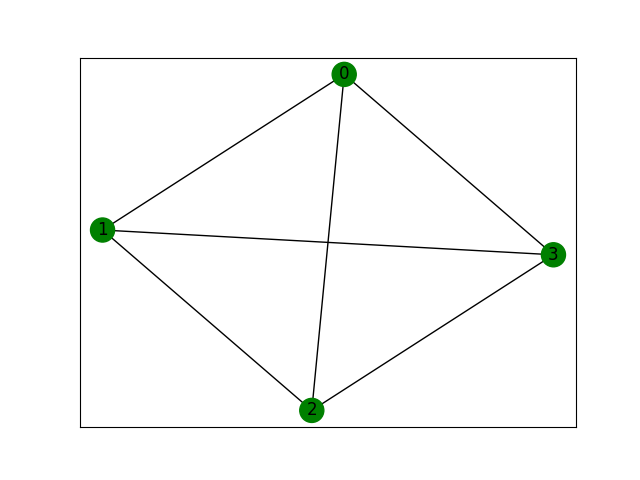
\includegraphics[width=0.5\textwidth]{images/4ngraph.png}
    \caption{4-n regular graph}
    \label{fig:4ngraph}
    \end{figure}
\end{minipage}
\begin{minipage}{0.45\textwidth}
Consider the following 4-n regular graph as shown in figure \ref{fig:4ngraph} for our analysis here.
Here, it is evident that the partitions with Maximum cost correspond to the following states : $\ket{0011}, \ket{0101}, \ket{0110}$ and the states with essentially the same partition but exchanging all the nodes, i.e, $\ket{1100}, \ket{1010}, \ket{1001}$. All of them have a cut of size 4.
\end{minipage}

In figure \ref{fig:UC1} it is evident that the probabilities do not change upon application of $U_C$ as discussed earlier.
It is only after the application of the \emph{mixing operator}, showed in \ref{fig:UB1}, that the probabilities change.
And we can also see that the states which correspond to higher cost have higher probabilities here in figure \ref{fig:UB1}.

\begin{figure}[H]
    \begin{minipage}{0.5\textwidth}
        \centering
        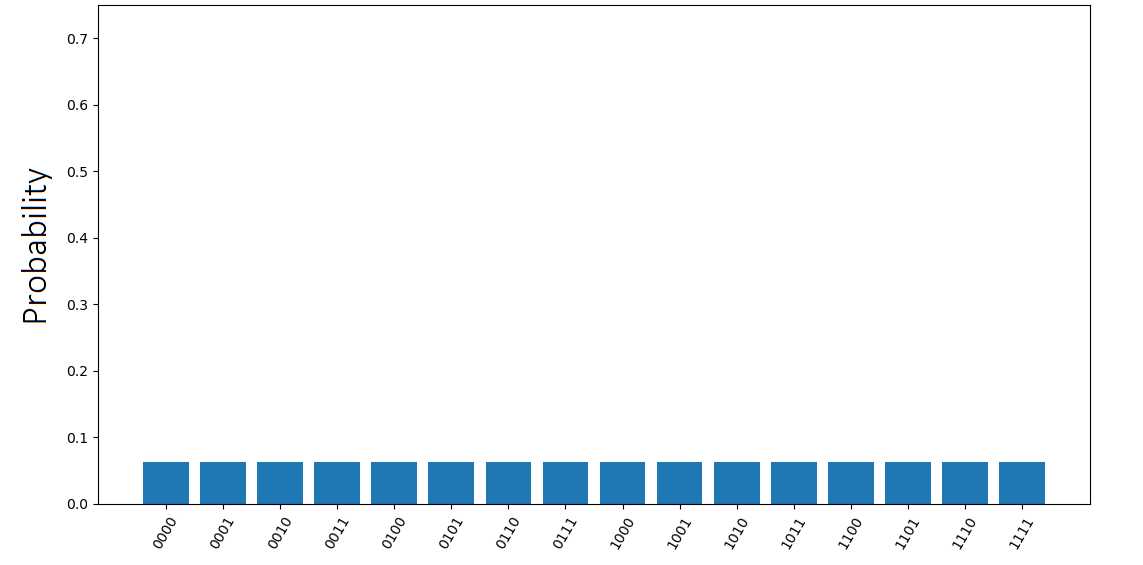
\includegraphics[width=\textwidth, height= 4.8cm]{1.png}
        \caption{Resulting state after $U_C$: $U_C\ket{+}^{\otimes 4}$\\
                $\gamma = 3.633$, $\langle C \rangle =3$}
        \label{fig:UC1}
    \end{minipage}
    \begin{minipage}{0.5\textwidth}
        \centering
        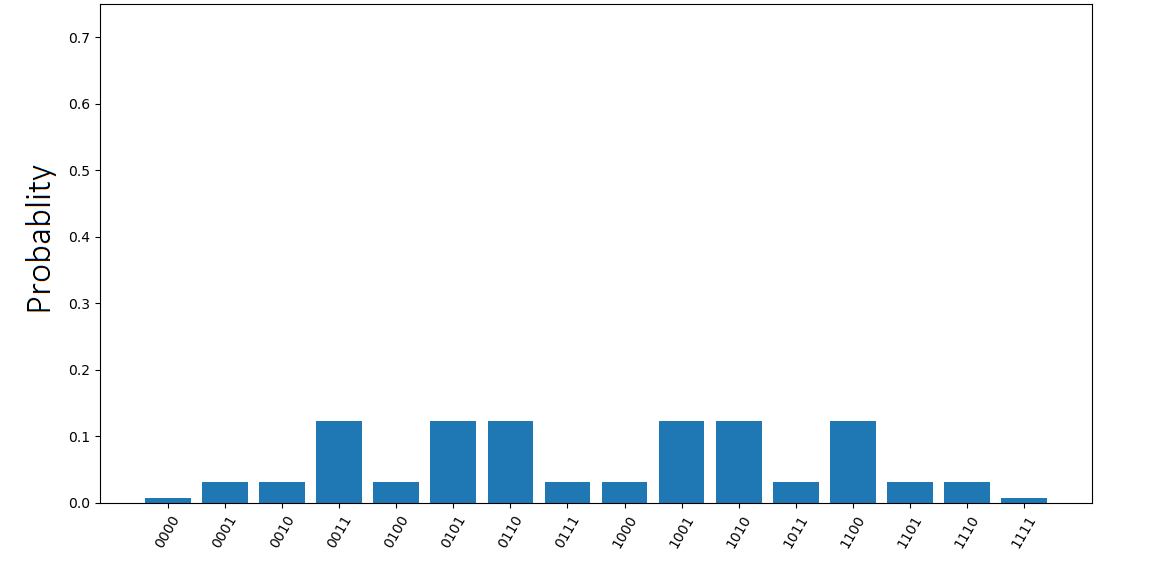
\includegraphics[width=\textwidth, height= 4.8cm]{2.png}
        \caption{Resulting state after $U_B$: $U_BU_C\ket{+}^{\otimes 4}$\\
                $\beta = 4.995$, $\langle C \rangle =3.798$}
        \label{fig:UB1}
    \end{minipage}
\end{figure}

We can see similar analysis for more than one layers. It can be seen that for an ideal case (without noise), as with the state vector simulator, the performance should monotonically increase with increasing p.
Say the approximation ratio after $p$ layers is $\alpha_p$, then,
$$\alpha_{p+1} \geq \alpha_p$$
since we can have for the $(p+1)^{th}$ layer, $(\beta_{p+1}, \gamma_{p+1}) = (0, 0)$.
And in that case, it is same as essentially applying only $p$ layers.
Note, that this is only true if there is no noise and we explore the performance in presence of noise further in the sections that follow.

For the same 4-n regular graph shown in figure \ref{fig:4ngraph}, we see the evolution of state vector for $p = 2$ layers.

\begin{figure}[H]
    \centering
    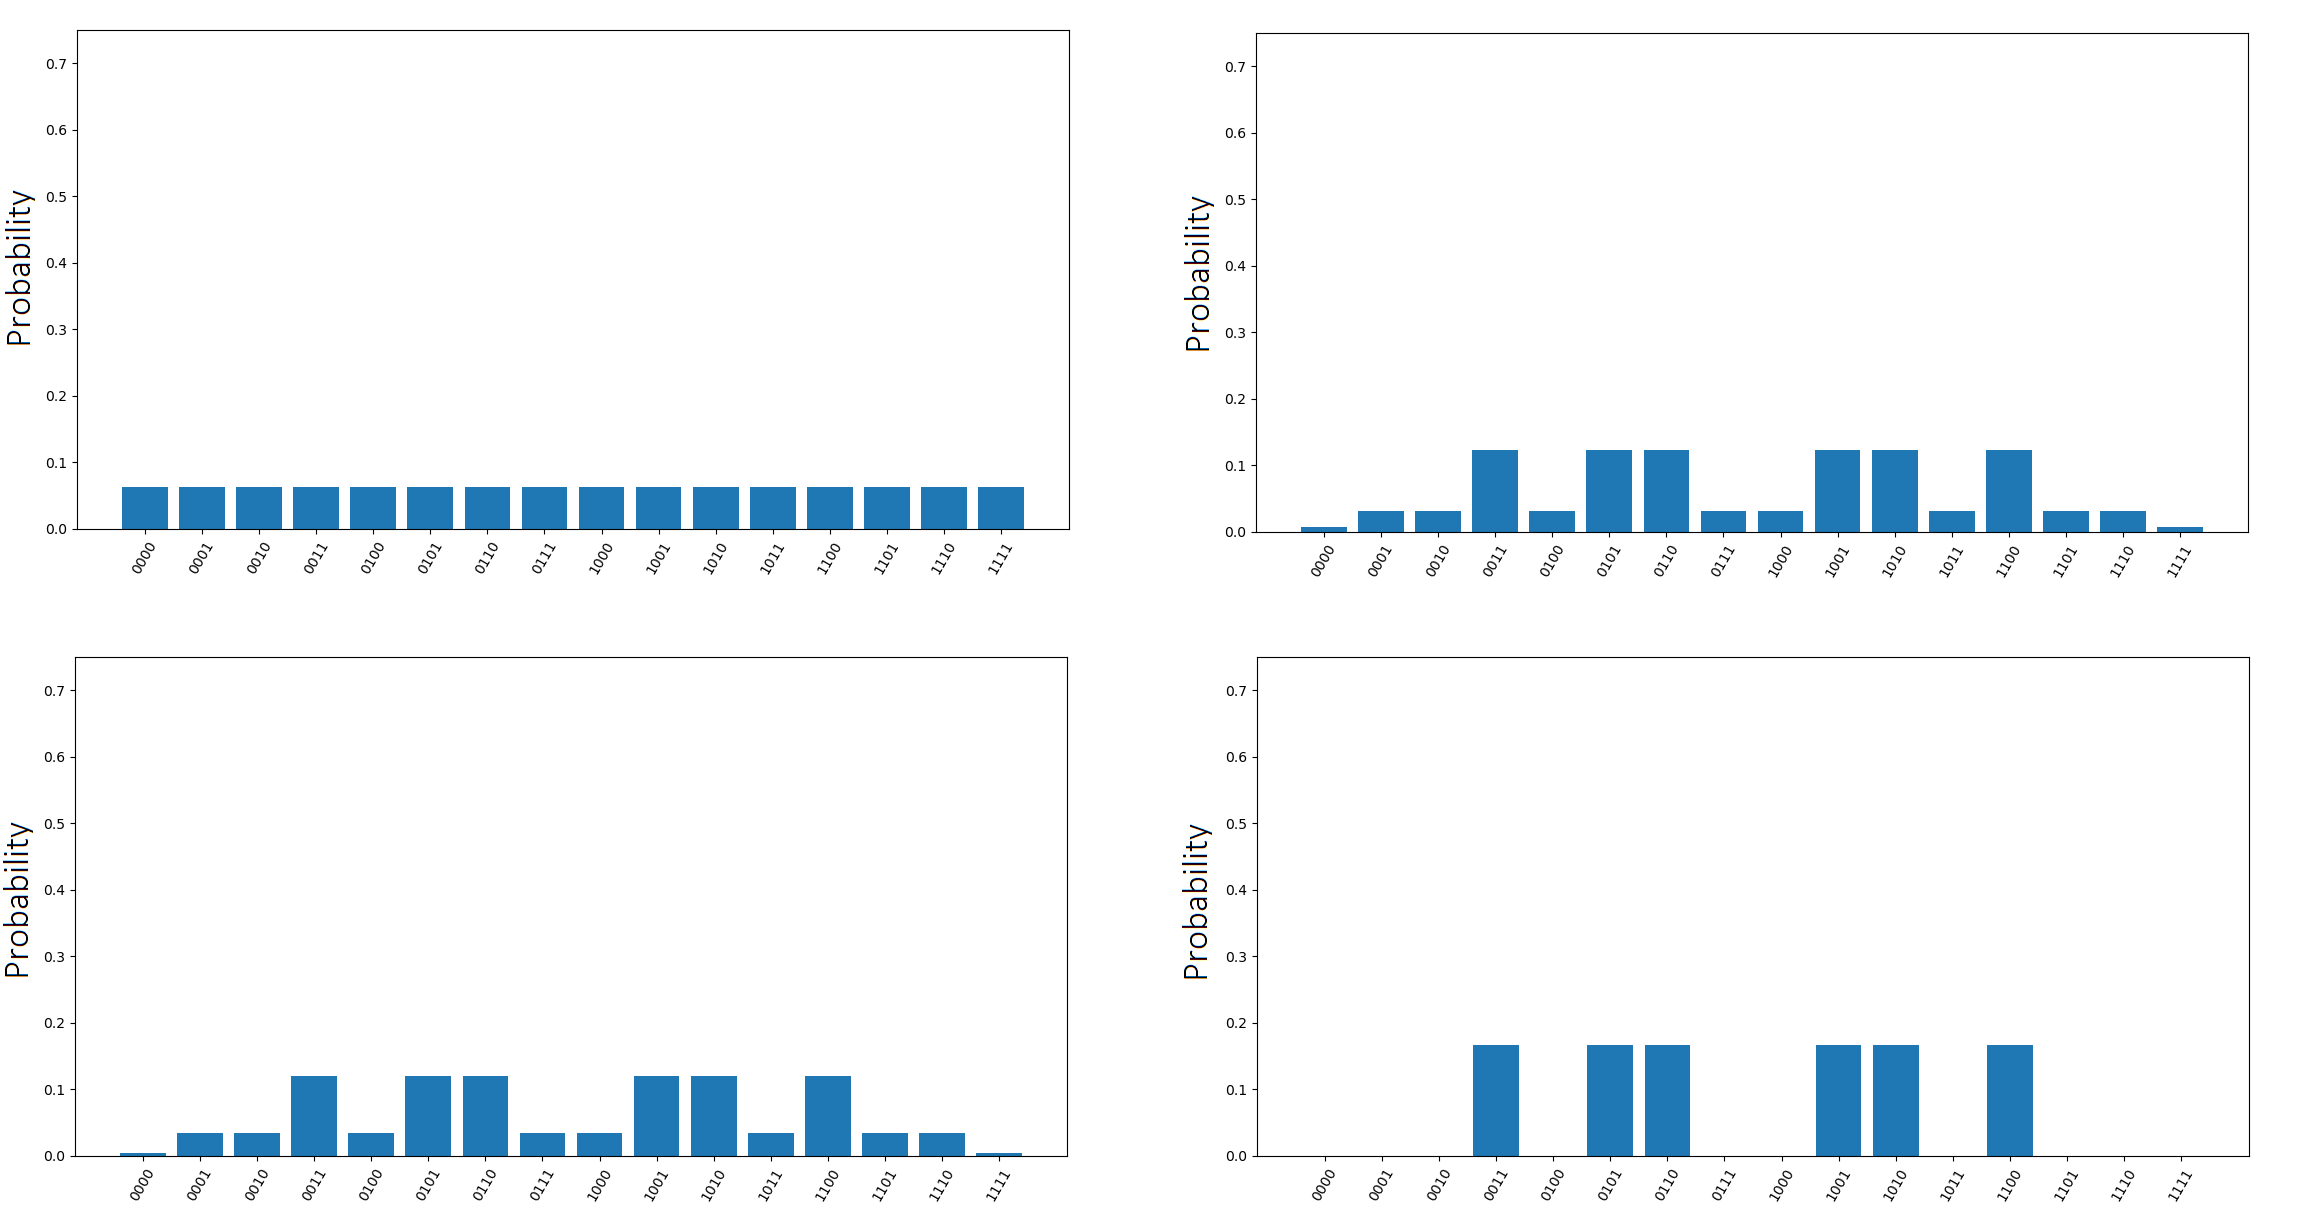
\includegraphics[width= \textwidth,  height= 7.9cm]{Figure_2.png}
    \caption{One possible evolution of state vector to the optimum solution for 4n regular graph for $p = 2$ layers\\
    $\vec{\gamma} = [3.633, 4.867]$, $\vec{\beta} = [4.995, 6.121]$ and $\langle C \rangle = 4$}
    \label{fig:stvc_lbl}
\end{figure}

We note that for $p = 2$, after applying the gates in both the \textit{layers}, with probability almost equal to 1, we get the states with the maximum cost. Thus, we always find the MaxCut in this case.
One interesting feature we see in figure \ref{fig:stvc_lbl}, is the that the optimizer keeps the same $\gamma_1$ and $\beta_1$ for both the cases i.e, when we had $p = 1$ and now that we have $p = 2$.
But this need not be the case. There could be other \textit{optimization paths} that the optimizer can take.
This can be seen in the following figure \ref{fig:my_label}
 
 \begin{figure}[H]
     \centering
     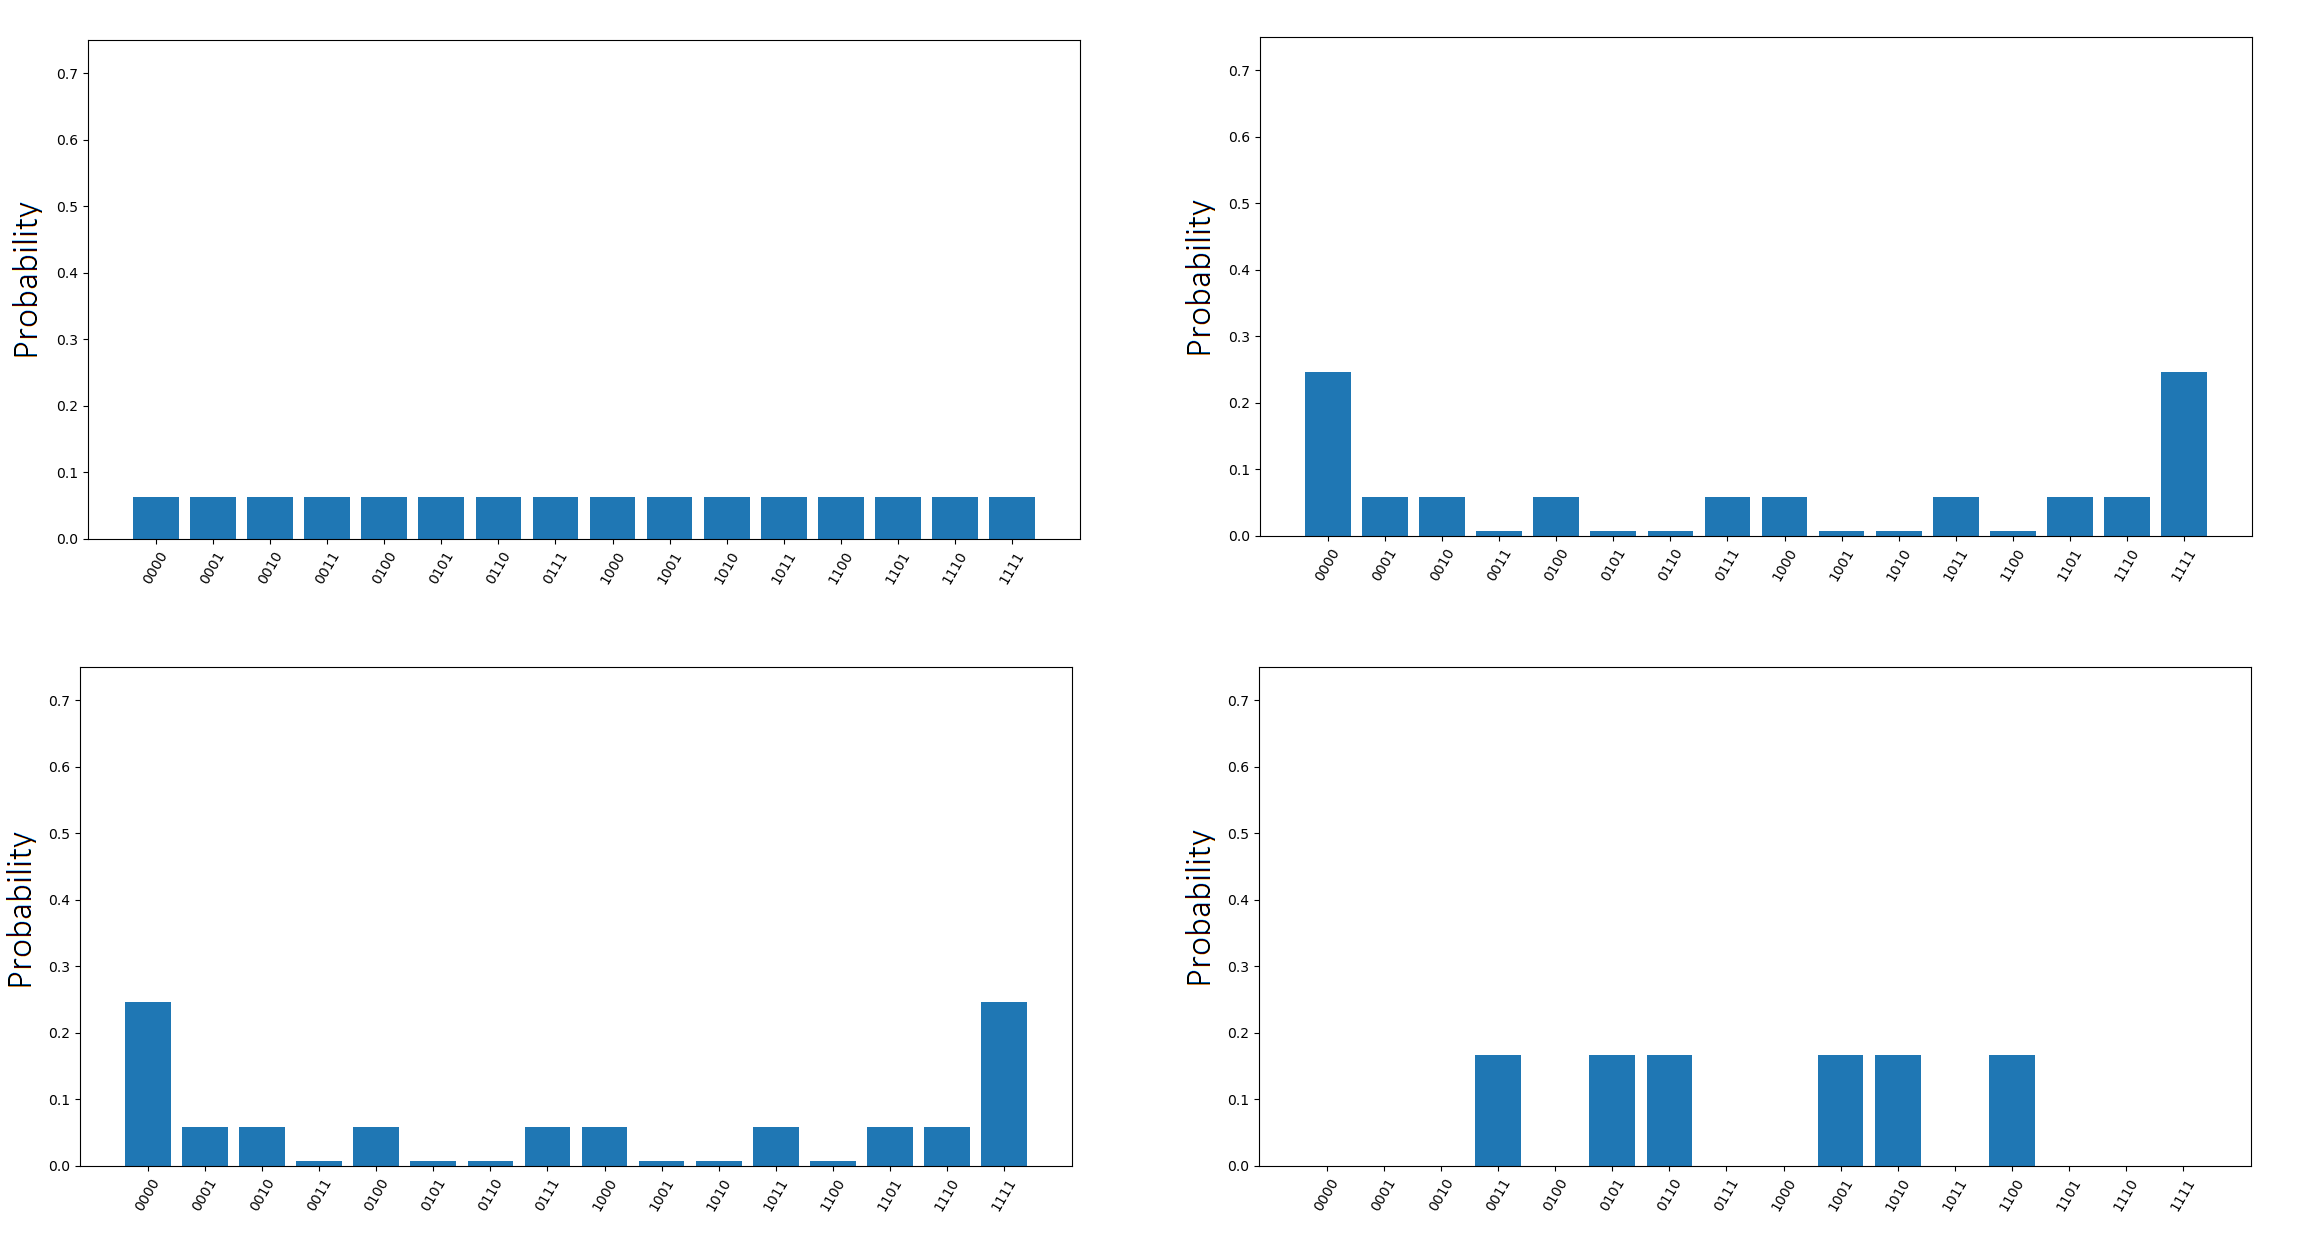
\includegraphics[width= \textwidth, height= 7.9cm]{Figure_1.png}
     \caption{Another evolution of state vector to the optimum solution for 4n regular graph for $p = 2$ layers\\
    $\vec{\gamma} = [5.718, 1.329]$, $\vec{\beta} = [5.545, 0.56]$ and $\langle C \rangle = 4$}
     \label{fig:my_label}
 \end{figure}
 
Thus, with different optimization paths taken, we can reach the same optimum solution.
 
 \begin{figure}[h]
    \begin{minipage}{0.33\textwidth}
        \centering
        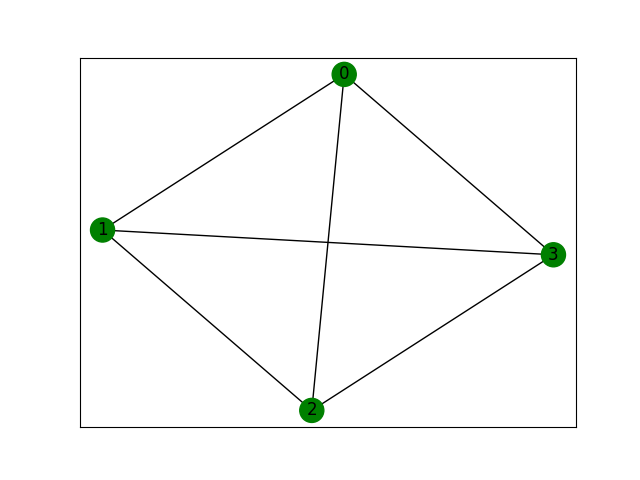
\includegraphics[width=\textwidth]{images/4ngraph.png}
        \caption{4-nodes regular graph}
        \label{fig:4n}
    \end{minipage}
    \begin{minipage}{0.33\textwidth}
        \centering
        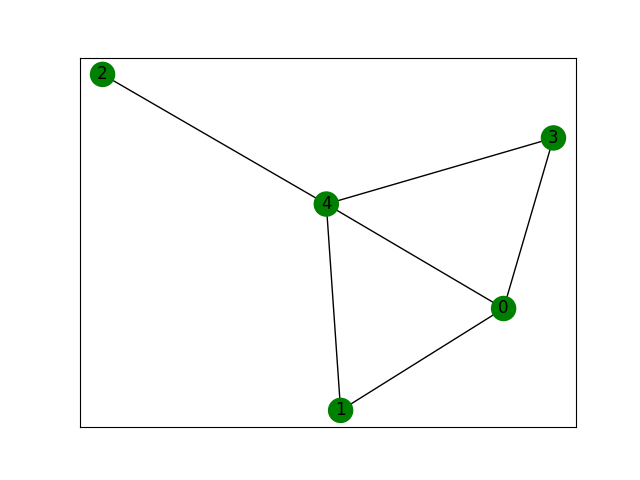
\includegraphics[width=\textwidth]{images/erdos renyi n = 5.png}
        \caption{5-nodes Erdos Renyi}
        \label{fig:er5}
    \end{minipage}
    \begin{minipage}{0.33\textwidth}
        \centering
        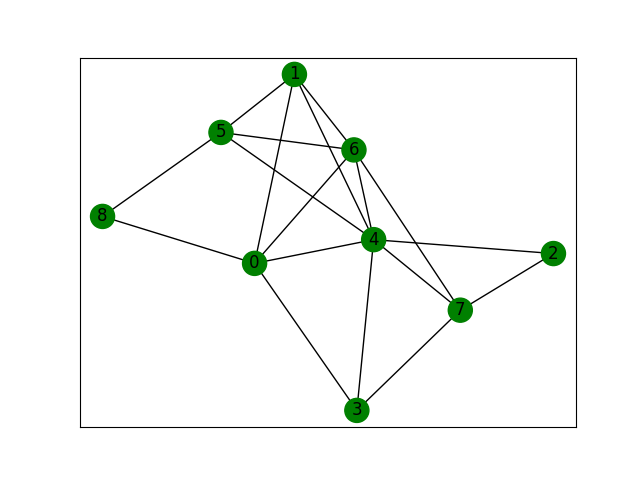
\includegraphics[width=\textwidth]{images/Erdos-Renyi graph.png}
        \caption{9-nodes Erdos Renyi}
        \label{fig:er9}
    \end{minipage}
\end{figure}

For the ideal case, we also look at other more complex graphs and see the performance of QAOA.
At the top of the page, in the figure \ref{fig:4n}, we have the 4n regular graph that we considered up until now. Additionally, in figure \ref{fig:er5} and \ref{fig:er9}, we see a 5-node and 9-node graph generated using the Erdos Renyi random graph model.
 \begin{wrapfigure}{l}{0.66\textwidth}
    \centering
    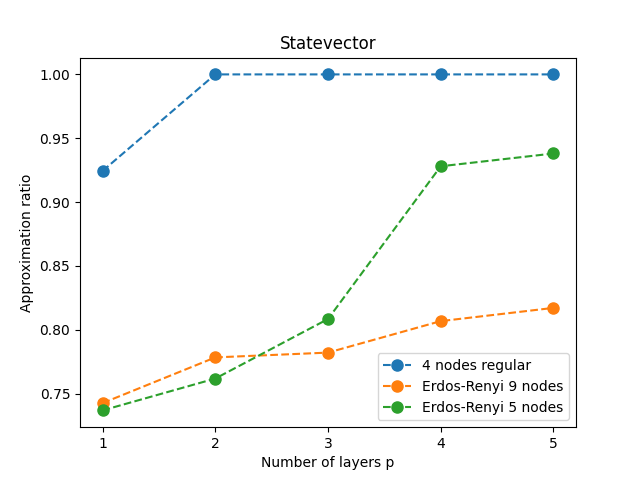
\includegraphics[width=0.66\textwidth]{images/StateVector.png}
    \caption{Comparison between the results for different graphs.}
    \label{fig:statevector_graph}
\end{wrapfigure}

As the figure on the left shows, the performance of the algorithm (measured as the ratio between the expectation value obtained and the actual max cut of that graph) is not as high for small values of p for more complex graphs.
We can also note that, as expected, the performance increases with the number of layers $p$.\\
Thus, for more complex problems, one would require sufficient number of layers to actually solve the MaxCut or any similar combinatorial optimization problem.
But, increasing $p$ is not only computationally expensive, but there are also errors which play a bigger role as circuit depth and complexity increases.

To finally include the noise that we have talked about until now, we can not use the StateVectorSimulator.
We use an actual quantum simulator next and analyse the result.

\section{QASM simulator}
\label{qasm_section}
We use QASM simulator provided by Qiskit and implement the algorithm.
We again consider the same 4n regular graph as earlier.
We use a simple noise model at first. We consider only depolarising error and see how the extent of depolarisation affects the performance. The depolarising error can be characterised as:

\[
    \rho \Rightarrow (1-\lambda)\rho + \lambda \frac{\mathds{1}}{d}\text{,}\quad \text{with } \rho = \ket{x}\bra{x}
\]
Here $\lambda \in [0, 1]$ is the \emph{depolarizing factor}. Greater the value of $\lambda$, greater is the depolarisation.

 \begin{wrapfigure}{r}{0.66\textwidth}
    \centering
    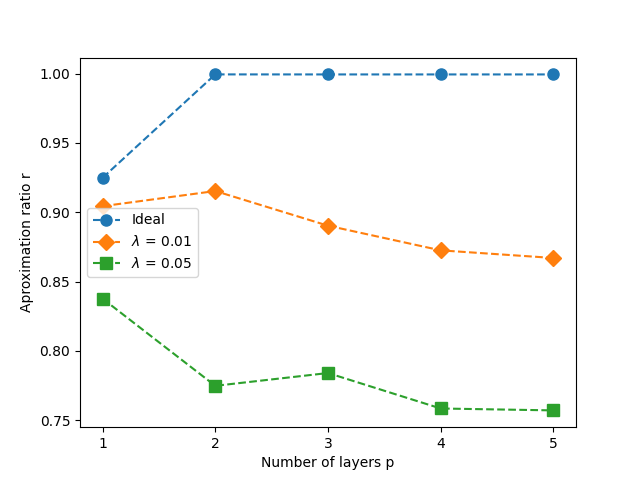
\includegraphics[width=0.66\textwidth]{images/depolarizing noise.png}
    \caption{Depolarizing noise running the algorithm for the regular 4-nodes graph.}
    \label{fig:dep_err_per}
\end{wrapfigure}
The figure \ref{fig:dep_err_per} on the right compares the performance for different values of $\lambda$.

Firstly we can see how QASM gives the same results for the ideal case that we observed in StateVector simulator earlier, as is expected.
But what this simulation reveals for noisy system is that the performance does not necessarily go up with increasing $p$.
We also see that for more noise, the algorithm is performing worse, as is expected.
Not only do the errors add up as the number of operations increase with the circuit depth increases, but as the circuit depth increases, the execution time also goes up and then we see more depolarisation.
We also see that for smaller values of $\lambda$, we get optimum performance for $p=2$ but for greater noise ($\lambda = 0.05$ here), we in fact get optimum performance for $p = 1$.
Tying this to our analysis in previous section for more complex systems \ref{fig:statevector_graph}, this implies that even though we need more number of layers for better performance, using more layers will be counterproductive since the increasing error due to noise disincentivizes using more layers, as we see here.

Thus far, we have only considered only depolarising error, we further consider more complex errors and try to \textit{mimic} a real quantum hardware.

\section{Fake Vigo}
\label{fakevigo_section}

The optimisation process in QAOA requires a high number of calls to the objective function. Therefore, before we run it on an actual hardware backend, it is practical to first run it on a simulator with a noise model as close to the actual noises as possible to be able to gauge the performance and to get an idea about what to expect. In this section we use a built in noise model provided with Qiskit called \texttt{FakeVigo}. This is a noise model based on the IBM's Quantum device \texttt{Vigo} and thus the name \texttt{FakeVigo}.


FakeVigo noise model includes the following errors:
\begin{itemize}
    \item \textbf{Single-qubit gate errors} consisting of a single qubit depolarizing error followed by a single qubit thermal relaxation error.
    \item \textbf{Two-qubit gate errors} consisting of a two-qubit depolarizing error followed by single-qubit thermal relaxation errors on both qubits in the gate.
    \item \textbf{Single-qubit readout errors} on the classical bit value obtained from measurements on individual qubits.
\end{itemize}

\newpage

 \begin{wrapfigure}{l}{0.66\textwidth}
    \centering
    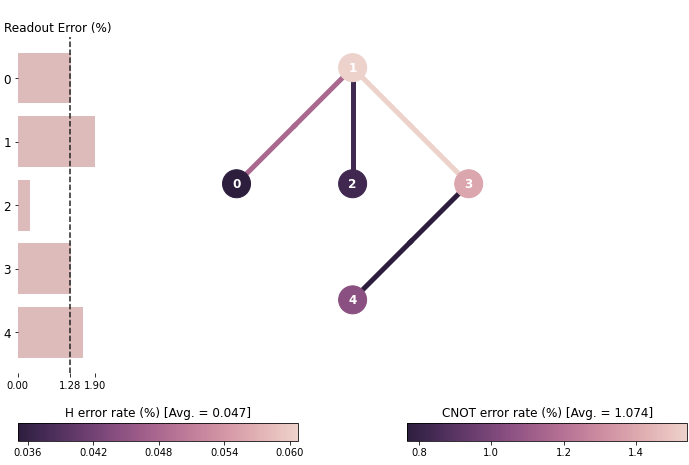
\includegraphics[width=0.5\textwidth]{images/fakeVirginMap.png}
    \caption{Fake Vigo error map provided by Qiskit.}
    \label{fig:error}
\end{wrapfigure}

Thermal relaxation takes in account the T1 time (also known as energy relaxation time) and T2 time (also known as dephasing time). These two parameters account for the overall decoherence error the qubit suffers. On figure \ref{fig:error} we can see a detailed error map provided by Qiskit which shows the error parameters and how they change for each qubit. Furthermore, the thermal relaxation, which are not included in the figure, are obtained from the documentation\cite{vigo_ref}.

Thus, we do similar analysis as we did for simple depolarising error and plot the results as shown in figure \ref{fig:4n_fakeV}.

Here we see that for a realistic noise model, the performance does not actually increase with increasing $p$ but it instead falls.
This points out the fact that our system is too erroneous and that the increase in performance due to more layers is not sufficient to overcome the decrease in performance due to errors.

\begin{figure}[h]
    \centering
    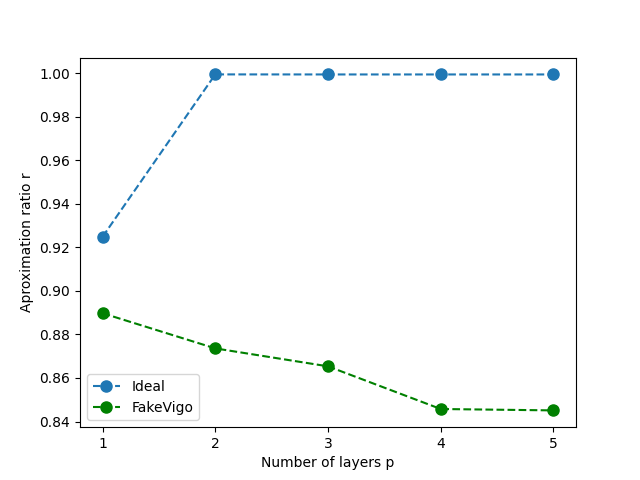
\includegraphics[width=0.5\linewidth]{images/4 node regular graph with fake vigo.png}
    \caption{Comparison of approximation ratio for \texttt{FakeVigo} and ideal case (no noise) for 4n regular graph for up to $p = 5$.}
    \label{fig:4n_fakeV}
\end{figure}

%%%%%%%%%%%%%%%%%%%%%%%%%%%%%%%%%%%%%%%%%%%%%%%%%%%%%%%%%%%%%%%%%%%%%%%%%%%%%%%%%%%%%%%%%%%%%%%%%%%%%
\section{Hardware Backend}
\label{hardware_section}

Up until now we have been running the algorithm on classical simulators. As a next step we will run it on real hardware. As mentioned earlier, we have chosen the IBM Quantum Experience's machine \textit{Vigo} \cite{vigo_ref}, a 5-qubit quantum processor (see figure \ref{vigo}). 

The first thing we need to realize is that in a real quantum computer not all the qubits are connected. This means that it is not possible to apply 2-qubit gates directly between any two arbitrary qubits. To apply 2-qubit gates between qubits that are not connected some intermediate gates (SWAP gates) are needed. This considerably increases the circuit depth and, as a consequence, the overall error. We will again apply our algorithm to the 4-n 3 regular graph, so it is easy to see that the shapes of the graph (figure \ref{fig:4ngraph}) and Vigo (figure \ref{vigo}) do not match, meaning that the compiler will indeed add intermediate SWAP gates that will increase the overload of the circuit.


In addition, we face another issue when running the algorithm on real backends: the time needed to run a job in IBM Quantum Experience. As most of the current backends nowadays, IBM's machines are only accessible via cloud. Therefore, when you submit a job to an IBM's machine it enters a queue with jobs from other users before eventual execution. The order in which these jobs are executed is decided through a fair-share queuing formula, which means that the more complex your job is the more time it will take to be executed. As QAOA is an optimization algorithm, it takes many evaluations to the objective function to reach the optimal value of all the $\gamma$ and $\beta$. Each of these evaluations of the objective function will be queued with a waiting time around 1-4 minutes, so the time needed to run the entire algorithm escalates very quickly with the number of layers.

Therefore, it is key to come up with ideas to reduce the number of function evaluations the optimizer takes. Many approaches have been taken in this direction, as for example in \cite{alam2020accelerating} where a machine  learning based approach is taken to accelerate the QAOA convergence through feature extraction. In this project we have addressed this problem with two different ideas: \textit{layer by layer optimization} and a \textit{smart choice of the optimizer}. 


 \begin{figure}
 
    \begin{minipage}{0.5\textwidth}
    \centering
    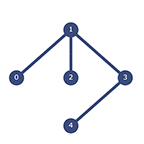
\includegraphics[width=.5\textwidth]{Vigo.png}  
  \captionsetup{width=.8\linewidth}
    \caption{Schematic representation of the connectivity of the qubits in Vigo. Retrieved from \cite{vigo_ref}}
    \label{vigo}
    \end{minipage}\begin{minipage}{0.5\textwidth}
    \centering
    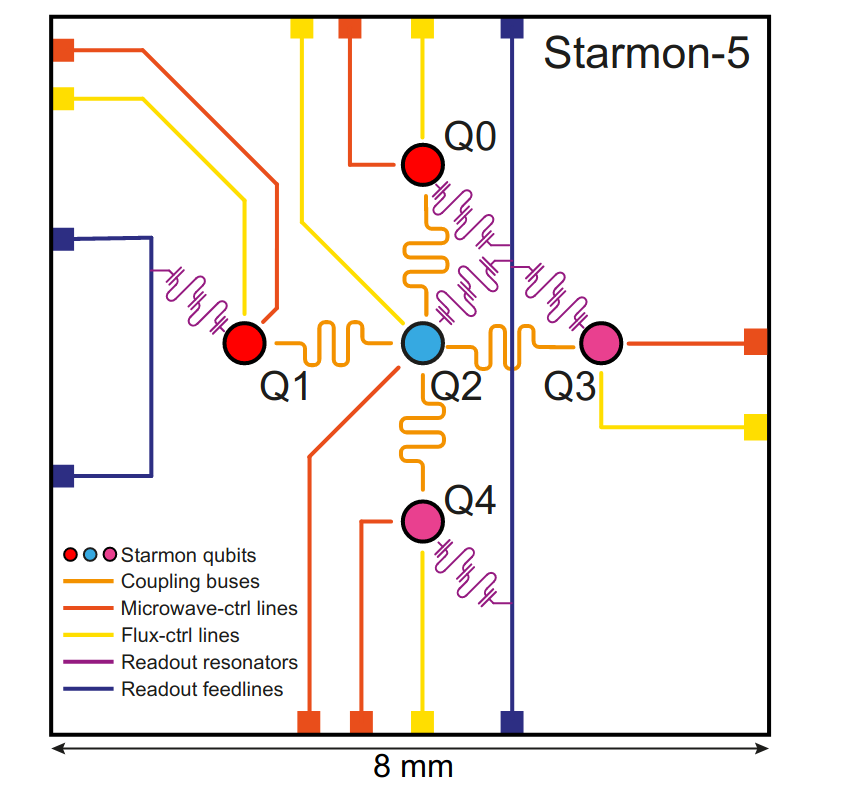
\includegraphics[width=.52\textwidth]{images/starmon5.png}   
  \captionsetup{width=.8\linewidth}
    \caption{Starmon 5 quantum processor. Retrieved from \cite{starmon_ref}}
    \label{starmon5}
    \end{minipage}

\end{figure}


\subsection{Layer by layer optmization}

Let's first consider the classical approach when running QAOA with $p$ layers. In this setting we have a circuit with $2p$ parameters, a $\gamma$ and a $\beta$ for each layer. Thus, the classical optimizer will optimize these $2p$ parameters all at once. This will be referred as \textit{standard optimization} from now on. Standar optimization works fine when $p$ is low, but the dimension of the solution parameter's space drastically increases for high $p$. This means the optimizer will likely need to compute many evaluations to the objective function. An illustration  can be seen in figure \ref{calls}, where the red line shows the number of calls made by the standard optimization for increasing $p$. 

\begin{figure}[h]
    \centering
    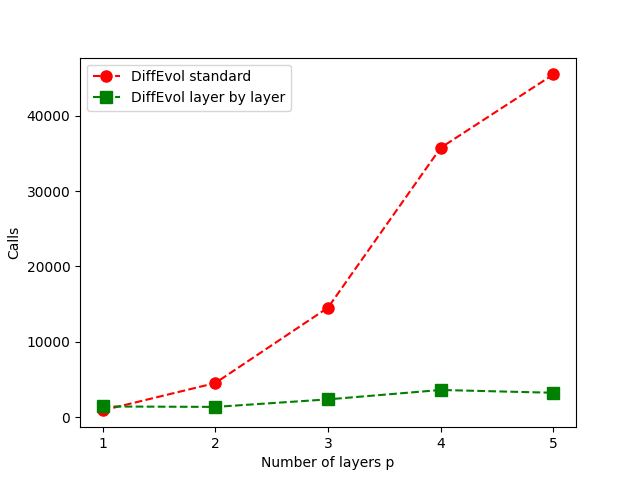
\includegraphics[width=0.5\linewidth]{images/Calls.png}    
    \caption{Number of calls to the objective function needed for standard and layer by layer optimization for increasing $p$}
    \label{calls}
\end{figure}

An alternative approach is the so called \textit{layer by layer} optimization. Let's again consider the case where we would like to run QAOA with $p$ layers. Withing this approach, we would first run the algorithm for $p=1$ and search for the optimum values of $\gamma_1, \beta_1$. Next, keeping the values for $\gamma_1, \beta_1$ fixed, we would run the algorithm for $p=2$ and optimize only the parameters for this layer $\gamma_2, \beta_2$. This process would be repeated $p$ times, optimizing the parameters of the ith-layer $\gamma_i \beta_i$ by keeping all the previous parameters  $\gamma_1, \beta_1 ... \gamma_{i-1}, \beta_{i-1}$ fixed. It is important to realize that now the dimension of the solution space is only 2 and not $2p$ like before, and that increasing $p$ does not imply that this dimension in increased, but rather that we will have to optimize $p$ times in a 2-dim solution space. Therefore, we would expect that the calls made to the objective function increases linearly with p. Indeed this can be seen in figure \ref{calls}.

% No we do not have any reference for layer by layer I think. It is something we came up with bro. That is the originality :P But on a serious note, I don't think there are references for that because it is not really QAOA anymore and this is a sacrifice we thought we would do.

\begin{figure}
    \centering
    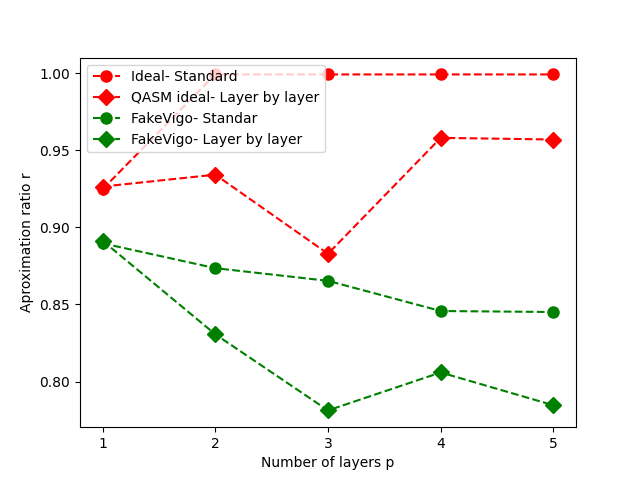
\includegraphics[width=0.6\linewidth]{images/layer by layer vs standard performance.png}
    \caption{Performance of the algorithm with standard and layer by layer optimization for increasing $p$. In red, for the QASM simulator with no noise and in green, for the FakeVigo simulator.}
    \label{performance layer standard}
\end{figure}

A final remark on the layer by layer optimization approach is that we are not considering the complete solution space but rather a subset of it. This means that the layer by layer optimization is not expected to reach a performance as high as the standard optimization. This is shown in figure \ref{performance layer standard}, where we compare the performance of the two optimization approaches in both the ideal QASM simulator and the FakeVigo simulator. Layer by layer optimization consistently achieves lower approximation ratios than the standard optimization for $p>1$ (for $p=1$ they are equivalent). 

One might be surprised to see, in figure \ref{performance layer standard}, that in the ideal case the performance drops for the ideal case in QASM for $p=3$. The performance in this ideal setting should be in principle at least as large as in the previous layer, since the optimizer should be able to choose $\gamma_3=0, \beta_3=0$, which would make the third layer to act as the identity, i.e. not perform any operations. The reason for this drop in $p=3$ is then probably due to the optimizer terminating the optimization before having found the optimal $\gamma_3, \beta_3$ as the maximum number of allowed iterations was reached.


\subsection{Choice of the optimizer}

There exists a wide variety of optimizers we can choose from. Current research is still vague on what optimizers will work best in this kind of hybrid quantum-classical algorithms like QAOA, so the choice of the optimizer usually takes an heuristic approach. Up until this section we used \textit{Differential-Evolution}, a global optimizer that has been shown to work well for QAOA \cite{alam2019analysis}. This is a global optimizer, which means it can avoid getting stuck in local minima, but on the other hand it usually takes many calls to the function. Other authors \cite{Lacroix_2020} have also used the local optimizers like \textit{Nelder-Mead} with satisfactory results. Additionally, Nelder-Mead needs to take less evaluation than Differential-Evolution. For this reason, Nelder-Mead was the chosen optimizer for running the algorithm in real backend


\subsection{Results}

We run QAOA for the Max-Cut on the 4-n 3-regular graph (figure \ref{fig:4ngraph}) in Vigo with up to 5 layers $(p=5)$. Even with the layer by layer optimization and using the Nelder-Mead optimizer, the whole code took around 2 days to run. Results can be seen in figure \ref{real_backend}. As expected, the overall performance for any $p$ in Vigo is lower than in FakeVigo, confirming that indeed this simulator heavily underestimates the errors in the real Vigo. On the other hand, FakeVigo did predict the qualitative behaviour of the algorith for $p>1$. Indeed we can see that, in the same way as in Vigo, the performance drops when adding more than one layer, unlike in the ideal case where the performance grows monotonically with $p$ (recall figure \ref{fig:statevector_graph}).
%I don't think we necessarily need a reference here. It can easily be seen that for greater p it should be at least as high as previous one. Maybe talk about that part earlier?


Additionally, we made use of QuTech's superconducting quantum processor, Starmon 5, consisting of 5 transmon qubits \cite{starmon_ref}. We were only able to run the algorithm for up to $p=3$ as the execution times in Starmon 5 when running deep circuits (recall that the depth of the circuit scales as $p$) were higher than in Vigo. The achieved performance in Starmon 5 was lower aswell. Error values aside, this fact is explained by the connectivity of the qubits in Starmon 5, which can be seen in figure \ref{starmon5}. It is easy to see that Vigo's topology is more adequate for the 4-n 3-regular graph, since less 2-qubit gates need to be applied between non connected qubits than in Starmon 5. This leads to more intermediate SWAP gates being applied, contributing to the overall error in the circuit. 


\begin{figure}
    \centering
    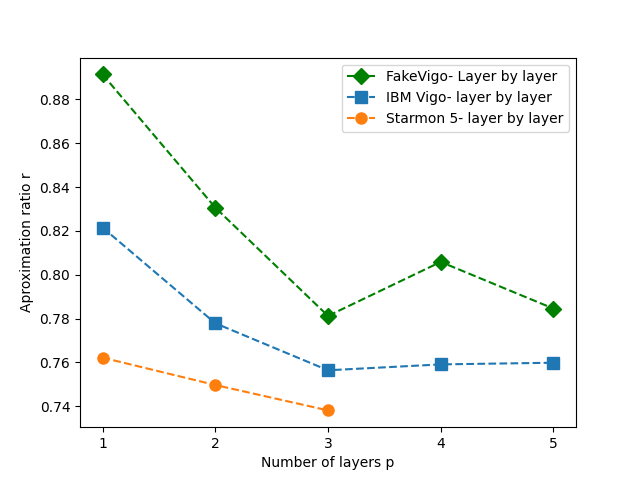
\includegraphics[width=0.6\linewidth]{images/starmon5 and vigo.png}    
    \caption{Performance of the algorithm in two real backends: Vigo from IBM Quantum Experience and Starmon 5 from QuTech, compared to that on the classical simulator FakeVigo.}
    \label{real_backend}
\end{figure}
%%%%%%%%%%%%%%%%%%%%%%%%%%%%%%%%%%%%%%%%%%%%%%%%%%%
The implementation of the project was done using the python library Qiskit. The code is available at \url{https://github.com/smitchaudhary/QAOA-MaxCut}.

%\chapter{Classical Approximation Algorithm}
%    \section{The Greedy Algorithm}

\section{Comparison between the two approximation algorithms}
\chapter{Discussion}
    
\section{Conclusions and future outlook}
In this project we have studied the Quantum Approximate Optimization Algorithm (QAOA) for the Max-Cut problem. We implemented the code from scratch and we run it for different classical simulators. We then made some modifications to the algorithm so that the number of evaluations to the objective function could be decreased, and finally we run it on two real quantum processors: Vigo from IBM Quantum Experience and Starmon 5 from QuTech. 

The performance of the algorithm in the most ideal case is promising, as we have seen in sections \ref{statevector_section} and \ref{qasm_section}, specially when we apply several layers of the algorithm. It quickly converges for the simplest graphs and gives a good approximation ration for more difficult graphs. But as we introduce noise, we observed that the errors in each layer quickly add up, and thus running the algorithm with many layers becomes counter-productive. For the real backends we have used, this optimal $p$ is 1, meaning that it is not efficient to run QAOA for $p>1$ in this devices. 

The results we have obtained, although very limited, point to a more general conclusion. The noise levels in current Quantum Computer only allow for QAOA to be run with a very low number of layers. For QAOA to present some advantage over classical algorithms, a high number of layers is likely to be needed \cite{Guerreschi_2019}. The future of this algorithm is therefore, like many other quantum algorithms, dependent on the improvement of the quantum hardware as many more qubits, with greater quality and connectivity, are needed. One of the reasons driving this interest in QAOA is the kind of problems it will solve. This kind of combinatorial optimization problems come up in many fields of industry, logistics, finance, science etc. Currently, QAOA is already being applied to some (very small) instances of real problems such as traffic control \cite{zhang2020qed} and flight scheduling \cite{Vikst_l_2020}. Still, the size of the analyzed data in this kind of papers is very small as the hardware is still veyr limited.

Nevertheless, the possible quantum advantage of QAOA over classical algorithms is not something that has been rigorously proven. In fact, M. Hastings published a paper in 2019 where a classical algorithm was mathematically shown to outperform QAOA for $p<1000$ \cite{hastings2019classical}. Therefore, although QAOA is thought to be very promising for the NISQ (Noisy Intermediate Scale Quantum) devices era, current research is casting some doubts on the subject. Despite this, there is a vast amount of scientific literature being produced about QAOA and, more generally, about Variational Quantum Circuits, making the future of this algorithms a hot topic within the quantum computing community. 




\printbibliography
%\bibliography{others/references.bib}
\end{document}